\documentclass[a4j]{jarticle}
    \usepackage[dvipdfmx]{graphicx}
    \usepackage[ top=25truemm,bottom=37truemm,left=25truemm,right=25truemm]
    {geometry}
    \usepackage{ascmac}
    \usepackage{amsmath}
    \usepackage{array}
    \usepackage{here}
    \usepackage{url}
    \usepackage{listings, jlisting}
    \usepackage{cases}
    \usepackage{txfonts}
    \usepackage[subrefformat=parens]{subcaption}
    \renewcommand{\lstlistingname}{リスト}
\lstset{language=c,
  basicstyle=\ttfamily\scriptsize,
  commentstyle=\textit,
  classoffset=1,
  keywordstyle=\bfseries,
  frame=tRBl,
  framesep=5pt,
  showstringspaces=false,
  numbers=left,
  stepnumber=1,
  numberstyle=\tiny,
  tabsize=4
}

\makeatletter
\def\@thesis{ネットワークプログラミング2}
\def\id#1{\def\@id{#1}}
\def\department#1{\def\@department{#1}}

\def\@maketitle{
\begin{center}
{\huge \@thesis \par} %修士論文と記載される部分
\vspace{10mm}
{\LARGE\bf \@title \par}% 論文のタイトル部分
\vspace{10mm}
{\Large \@date\par}	% 提出年月日部分
\vspace{20mm}
{\Large \@department \par}	% 所属部分
{\Large 学籍番号 \@id \par}	% 学籍番号部分
\vspace{10mm}
{\Large 氏名 \@author}% 氏名 
\end{center}
\par\vskip 1.5em
}

\title{自由課題}
\date{提出期限 2021年7月27日 14:20}
\department{組番号 409}
\id{17406}
\author{金澤雄大}

    \begin{document}
    \maketitle
    \thispagestyle{empty}
    \clearpage
    \addtocounter{page}{-1}
    \section{目的}
    ネットワークプログラミング2で学習した内容への理解を深めるために自由課題として製作物を作成することを目的とする.

    \section{製作物の説明}
    本章では製作物の説明として, 製作物の概要, 花札の基礎と用語, こいこいのルールの3つについて述べる.
    \subsection{製作物の概要}
    製作物として同期通信を利用して, 花札で遊べるゲームの1つである「こいこい」を作成した. こいこいは2人または3人で同じ絵柄の札を揃えて役を作るカードゲームで, ここでは2人での対局を想定している.
    また実装したこいこいのルールは任天堂のルール\cite{nintendo}を参考に, 一部プログラミングがしやすいように改変した.

    \subsection{花札の基礎と用語}
    花札の基礎と用語について説明する. 花札のカードは全48枚の札から構成されている. 札には1月から12月までの札が各4枚ずつ存在する. 各月の札の絵柄は図\ref{jan}~図\ref{dec}に示す通りである.
    札は月とは別に描かれている絵の種類で光札, タネ札, タン札, カス札の4種類に分けられる. 光札は最もレア度の高い札で1月の鶴が描かれている札, 3月の桜と幕が描かれている札, 8月の月が描かれている札, 11月の小野道風にカエル
    が描かれている札, 12月の桐に鳳凰が描かれている札の5枚のみである. タネ札は光札以外で動物や橋, 盃(さかずき)が描かれている札である. タン札は短冊が描かれている札である. カス札は植物のみが描かれている札である. 間違えやすい
    札として11月のカス札がある. 11月のカス札は黒と赤で構成されていて, 太鼓のようなものが描かれているがカス札である. 例外として9月のタネ札(盃が描かれている札)はカス札とタネ札の両方としてカウントする.
    
    \begin{figure}[H]
    \centering
    
\includegraphics[scale=1.5]{./img/jan.eps}
    \caption{1月 松に鶴}
    \label{jan}
    \end{figure}

    \begin{figure}[H]
    \centering
    
\includegraphics[scale=1.5]{./img/feb.eps}
    \caption{2月 梅にうぐいす}
    \label{feb}
    \end{figure}

    \begin{figure}[H]
    \centering
    
\includegraphics[scale=1.5]{./img/mar.eps}
    \caption{3月 桜に幕}
    \label{mar}
    \end{figure}

    \begin{figure}[H]
      \centering
      
\includegraphics[scale=1.5]{./img/apr.eps}
      \caption{4月 藤にほととぎす}
      \label{apr}
      \end{figure}
  
      \begin{figure}[H]
      \centering
      
\includegraphics[scale=1.5]{./img/may.eps}
      \caption{5月 菖蒲(アヤメ)に八ツ橋}
      \label{may}
      \end{figure}
  
      \begin{figure}[H]
      \centering
      
\includegraphics[scale=1.5]{./img/jun.eps}
      \caption{6月 牡丹に蝶}
      \label{jun}
    \end{figure}

    \begin{figure}[H]
      \centering
      
\includegraphics[scale=1.5]{./img/jul.eps}
      \caption{7月 萩に猪}
      \label{jul}
      \end{figure}
  
      \begin{figure}[H]
      \centering
      
\includegraphics[scale=1.5]{./img/aug.eps}
      \caption{8月 ススキに月・雁}
      \label{aug}
      \end{figure}
  
      \begin{figure}[H]
      \centering
      
\includegraphics[scale=1.5]{./img/sep.eps}
      \caption{9月 菊に盃(さかずき)}
      \label{sep}
      \end{figure}

    \begin{figure}[H]
      \centering
      
\includegraphics[scale=1.5]{./img/oct.eps}
      \caption{10月 紅葉に鹿}
      \label{oct}
      \end{figure}
  
      \begin{figure}[H]
      \centering
      
\includegraphics[scale=1.5]{./img/nov.eps}
      \caption{11月 小野道風にカエル, 柳にツバメ}
      \label{nov}
      \end{figure}
  
      \begin{figure}[H]
      \centering
      
\includegraphics[scale=1.5]{./img/dec.eps}
      \caption{12月 桐に鳳凰}
      \label{dec}
      \end{figure}

    \subsection{こいこいのルール}
      こいこいは花札を使用するゲームの1つである. 対局は2人または3人で行うが, ここでは2人で対局を行うときのルールについて説明する.
      こいこいは12回親と子を変えて対局し, 12回目の対局が終了したときに得点が高いほうが勝利するというルールである. \\
       対局手順について説明する. 1回目の対局では, はじめに親と子を決める. 親と子の決め方はまず, 48枚全ての札を裏返してシャッフルする. 次に親(先攻)と子(後攻)を決めるために, シャッフルした札から1枚ずつめくる. 
      めくった札の月が早いほうが親, 遅いほうが子である. 月が同じときは親子決めをやり直す. 親子が決まったら, 親が全ての札を裏返してシャッフルする. そして親が親, 子, 場にシャッフルした札を
      配る. 親と子は裏向き, 場は表向きで札を配る. 残った札は山札として裏向き重ねて置いておく. これで対局を始める準備ができた. また2回目以降の対局は親と子を交互に交代する. \\
       対局は親のターンから始まり, 親のターンが終わると子, 子のターンが終わると再び親のターンに戻る形式である. ターン中の行動は図\ref{turn-flow}のフローチャートの通りである.
      図\ref{turn-flow}の「こいこい」とはまだゲームを続けるかやめるかを選択することである. 「こいこい」を宣言すると相手のターンになり, 「あがり」を宣言すると対局が終了し, 
      こいこいを宣言した側の勝ちとなる. こいこいを宣言した後に相手の役(後述)ができると相手の役の得点が2倍になるためこいこいするかどうかは慎重に判断する必要がある.

      \begin{figure}[H]
      \centering
      \includegraphics[scale=1.8]{./img/turn-flow.eps}
      \caption{ターン中の行動手順}
      \label{turn-flow}
      \end{figure}

      役について説明する. 役とは手元に特定の札が揃ったときに自分の得点になり, こいこいするかどうかを決めるためのものである. 今回は次に示す11個の役を実装した. 
      ここに示す以外の役(例:手四, くっつき)もあるがここではそれらの役の判定は行わないものとする. また, 自分の役が7点以上になると得点が2倍になるというルールがある.
      このルールがあるため12月戦で点数を稼ぐためには2つ以上の役を作って7点以上稼ぐことで得点を伸ばすことができる.
      \begin{itemize}
        \item 五光(10点) : 光札5枚が全て揃う.
        \item 四光(8点) : 11月の光札を除く光札4枚が揃う.
        \item 雨四光(7点) : 11月の光札とそれ以外の光札3枚が揃う.
        \item 三光(5点) : 11月の光札を除く光札3枚が揃う.
        \item 花見で一杯(5点) : 3月の光札, 9月のタネ札が揃う.
        \item 月見で一杯(5点) : 8月の光札, 9月のタネ札が揃う.
        \item 猪鹿蝶(5点) : 6月, 7月, 10月のタネ札3枚が揃う.
        \item 赤短(5点) : 1月, 2月, 3月のタン札3枚が揃う.
        \item 青短(5点) : 6月, 9月, 10月のタン札3枚が揃う.
        \item タネ : タネ札5枚で1点, 1枚増えるごとに1点追加.
        \item タン : タン札5枚で1点, 1枚増えるごとに1点追加.
        \item カス : カス札10枚で1点, 1枚増えるごとに1点追加.
      \end{itemize}
      

    \section{実行環境とビルド方法}
    本章では, 実行環境, ファイル構成, ビルド方法の3つについて述べる.
    \subsection{実行環境}
    表\ref{env}に実行環境を示す. OpenGLとGLpngは4年次にプログラミング演習で使用したものを用いる.  
    \begin{table}[H]
        \caption{実行環境}
      \label{env}
      \begin{center}
          \begin{tabular}{c|l}\hline
            CPU & Intel(R) Core(TM) i7-6500U 2.50GHz  \\ 
            メモリ & 16.0GB DDR4 \\
            OS & Microsoft Windows 10 Home \\
            gcc &  version 9.3.0 \\
            make & version 4.3 \\ \hline
          \end{tabular}
      \end{center}
      \end{table}

    \subsection{ファイル構成}
    リスト\ref{files}に製作したゲームのファイル構成を示す. mylibディレクトリは授業中に作成したソケット通信用のライブラリである. 花札を実現するプログラムは
    mainディレクトリに入っている. さらにmainディレクトリ内にcardディレクトリがあり札の画像ファイルを格納している.
    \begin{lstlisting}[basicstyle=\ttfamily\footnotesize, frame=single,label=files,caption=ファイル構成]
5J_hanahuda
├── main
│   └── card
├── mylib
├── readme_img
└── readme.md
    \end{lstlisting}

    \subsection{ビルド方法}
ビルド方法について説明する. Google Driveからj17406.tar.gzをダウンロードして解凍した状態とする. まず, mylibディレクトリで
makeコマンドを実行してソケット通信用のプログラムをコンパイルする. 次にmainディレクトリでmakeコマンドを実行して花札を実行するプログラムをコンパイルする.
コンパイルができたら, s.exeとc.exeを実行すると対局が始まる.

    \section{プログラムの説明}
    本章ではserver.c, client.c, hanahuda.cの3つのプログラムの説明について述べる.
    \subsection{server.c}
    サーバー端末で動作するserver.cについて説明する. リスト\ref{server}にserver.cのプログラムを示す.
    リスト\ref{server}の10行目から28行目はOpenGLの処理である. 12行目から14行目ではウィンドウの生成を行っている.  
    16行目から21行目で動的な画面の描画, ウィンドウサイズの変更, キーボード, マウス処理のためにコールバック関数登録をしている.
    23行目から28行目ではアルファチャネルの有効化と背景色の変更の処理を行っている. 29行目から31行目では, サーバーのセットアップの処理
    を行っている. セットアップが失敗した場合は実行を終了する. 34行目では対局の初期化を行っている. game\_init関数の処理内容は
    4.3章のhanahuda.cで説明する. 最後に37行目でOpenGLのメインループに入る処理を行う. サンプルの五目並べのプログラムでは
    while文を用いたメインループでゲームの進行を行ったが, この処理をOpenGLに置き換えることでグラフィカルなゲームを実現している.
    \begin{lstlisting}[basicstyle=\ttfamily\footnotesize, frame=single,label=server,caption=server.c]
#include<stdio.h>
#include "hanahuda.h"
#include<GL/glut.h>
#include <GL/glpng.h>

int main(int argc,char **argv){
    int soc;
    // 初期化処理
    // 引数処理
    glutInit(&argc,argv);
    // 初期Windowサイズ設定
    glutInitWindowSize(WINDOW_W,WINDOW_H);
    // 新規Window作成
    glutCreateWindow("hanahuda_host");
    // 関数登録
    glutDisplayFunc(Display);
    glutReshapeFunc(Reshape);
    glutKeyboardFunc(Keyboard);
    glutMouseFunc(Mouse);
    glutPassiveMotionFunc(PassiveMotion);
    glutTimerFunc(500,Timer,0);
    //  テクスチャのアルファチャネルを有効にする設定
    glEnable(GL_BLEND);
    glBlendFunc(GL_SRC_ALPHA, GL_ONE_MINUS_SRC_ALPHA);
    glTexEnvf(GL_TEXTURE_ENV, GL_TEXTURE_ENV_MODE, GL_MODULATE);
    // display初期化
    glutInitDisplayMode(GLUT_RGBA);
    glClearColor(0.28,0.48,0.32,1.0);
    if( (soc=setup_server(PORT))==-1){
        exit(1);
    }

    // ゲーム初期化
    game_init(soc,0);

    // glutのメインループ
    glutMainLoop();
    return 0;
}
          \end{lstlisting}

    \subsection{client.c}
    クライアント端末で動作するclient.cについて説明する. client.cのプログラムをリスト\ref{client}に示す. 基本的な処理の流れはserver.cと同じである. 
    server.cとの違いは31行目から38行目である. 30行目および31行目では接続するホスト(サーバー)名を入力させる処理を行っている. ホスト名は「localhost」,「192.168.10.4」
    のように入力する. 33行目で実行しているchop\_newline関数はmylibディレクトリで定義されている関数で
    入力した文字列の末尾の改行文字をナル文字に置換する機能を持つ. 36行目から38行目では入力されたホストのIPアドレスをもとにクライアントのセットアップの処理を行っている.
    \begin{lstlisting}[basicstyle=\ttfamily\footnotesize, frame=single,label=client,caption=client.c]
#include<stdio.h>
#include "hanahuda.h"
#include<GL/glut.h>
#include <GL/glpng.h>

int main(int argc,char **argv){
    int soc;
    char hostname[64];
    // 初期化処理
    // 引数処理
    glutInit(&argc,argv);
    // 初期Windowサイズ設定
    glutInitWindowSize(WINDOW_W,WINDOW_H);
    // 新規Window作成
    glutCreateWindow("hanahuda_client");
    // 関数登録
    glutDisplayFunc(Display);
    glutReshapeFunc(Reshape);
    glutKeyboardFunc(Keyboard);
    glutMouseFunc(Mouse);
    glutPassiveMotionFunc(PassiveMotion);
    glutTimerFunc(500,Timer,0);
    //  テクスチャのアルファチャネルを有効にする設定
    glEnable(GL_BLEND);
    glBlendFunc(GL_SRC_ALPHA, GL_ONE_MINUS_SRC_ALPHA);
    glTexEnvf(GL_TEXTURE_ENV, GL_TEXTURE_ENV_MODE, GL_MODULATE);
    // display初期化
    glutInitDisplayMode(GLUT_RGBA);
    glClearColor(0.28,0.48,0.32,1.0);
    //サーバーのホスト名の入力
    printf("Input server's hostname: ");
    fgets(hostname,HOSTNAME_LENGTH,stdin);
    chop_newline(hostname,HOSTNAME_LENGTH);

    //接続完了まで
    if((soc = setup_client(hostname,PORT)) == -1){
        exit(1);
    }

    // ゲーム初期化
    game_init(soc,1);
    
    // glutのメインループ
    glutMainLoop();

    return 0;
}
          \end{lstlisting}

    \subsection{hanahuda.c}
    本節ではhanahuda.cにおける構造体および関数の説明について述べる.
    \subsubsection{札の処理}
    札の扱いと処理について説明する. 札はリスト\ref{cardstruct}に示すcard構造体の配列で定義されている. card構造体は
    月, 画像ファイルの番号, 札の種類の3つをメンバとして持っている.
    \begin{lstlisting}[basicstyle=\ttfamily\footnotesize, frame=single,label=cardstruct,caption=card構造体]
// 札用の構造体
struct cardstruct{
    int month; // 1-12
    int num; // imgの番号
    int rank; //1-4, 4:光札,3:タネ札,2:短冊札,1:カス札
};
typedef struct cardstruct card;
// 札用の構造体の配列を定義
static card cards[CARD_NUM];      
    \end{lstlisting}
    次に山札や場札から出すときの処理について説明する. 山札と手札は札を出す, 場札は札の出し入れの処理を行う必要がある.
    また獲得した札を保持する配列が必要である. これらの処理を行うために, javaにおけるsetterとgetterにあたる関数を用意した.
    リスト\ref{setget}に山札, 場札, 手札, 獲得した札の配列に札を出入力する関数を示す. 関数名がpopで始まる関数は札を管理する配列から
    札を取り出す関数, pushで始まるものは札を入力する関数である. 
    \begin{lstlisting}[basicstyle=\ttfamily\footnotesize, frame=single,label=setget,caption=札の入出力をする関数]
// 山札から札を出す処理
// 札のインデックスを返す
int popDeck(void){
    deck_num++;
    return deck[deck_num-1];
}

// 場に札を入れる処理
void pushPlace(int c){
    place[place_num++]=c;
}

// 場から札を出す処理
int popPlace(int index){
    int i;
    int tmp=place[index];
    for(i=index+1;i<place_num;i++){
        place[i-1]=place[i];
    }
    place[i-1]=-1;
    place_num--;
    return tmp;
}

// 手札から札を出す処理
int popHandCard(int index){
    int i;
    int tmp;
    if(role==0){ // 親のとき
        tmp = mycard[index];
        for(i=index+1;i<mycard_num;i++){
            mycard[i-1]=mycard[i];
        }
        mycard[mycard_num-1]=-1;
        mycard_num--;
    }else{ // 子のとき
        tmp = peercard[index];
        for(i=index+1;i<peercard_num;i++){
            peercard[i-1]=peercard[i];
        }
        peercard[peercard_num-1]=-1;
        peercard_num--;        
    }
    return tmp;    
}

// 持ち札に札を入れる処理
void pushgetCard(int c){
    if(role==0){
        mygetcard[mygetcard_num]=c;
        mygetcard_num++;
    }else{
        peergetcard[peergetcard_num]=c;
        peergetcard_num++;
    }
} 
    \end{lstlisting}

    \subsubsection{ゲームの初期化処理}
    ゲームの初期化処理について説明する. ゲームの初期化はリスト\ref{initgame}の3行目から15行目に示すgame\_init関数を実行することで行われる.
    game\_init関数の内部では, まず6行目で親と子の区別をするための変数roleに引数から受け取った値を代入する処理を行っている. 親のときリスト\ref{server}の34行目に示したように, 
    roleを0, 子のときリスト\ref{client}の41行目で示したようにroleを1に設定している. \\
     8行目では配列の初期化を行う関数であるarray\_init関数を実行している. array\_init関数の定義は44行目から46行目である. 9行目ではreadImg関数を実行している.
    readImg関数の定義は18行目から41行目である. readImg関数ではcardディレクトリに置いたある札の画像を取得しcardimg配列に代入する処理を行っている. カード名をsprintf関数で指定してから
    指定されたパスの画像を取得するpngBind関数を実行することで48枚の札の取得を実現している.\\
     11行目から14行目では山札をシャッフルして場と手札に札を配る処理を行っている. 山札のシャッフルは83行目から100行目に定義したshuffle関数で行っている. 花札の札には重複がないため乱数をランダムに代入して
    山札を生成することができない. そこで0から47までの数字が1つずつ入った配列を生成し, ランダムに2つを選択して交換する処理を何度か繰り返すことで重複のないランダムなリストを生成している.
    交換回数は10000回としている. 山札の設定が終わったから104行目から127行目に示すarrangeCard関数を用いて場と2人の手札にそれぞれ8まいずつ札を配る処理を行っている. このとき, 場に3枚以上同じ月の札がでたら
    山札のシャッフルと札の分配をやり直すかどうかの判定を行い, やり直しの必要があるときは1を返すようにしている. game\_init関数関数では返り値が0になるまでループさせることで
    場に取れない札がでることを防止している. なお本来の対局では場に3枚同じ札が出た時は残りの1枚を場に出したときに4枚すべて獲得できる, または場に出ている3枚から1枚をランダムに山札に戻して別の1枚をだし, 山札をシャッフルしなおすという
    ルールになっている. 場に4枚同じ札がでたときのルールは公式なものはないが場と山札をシャッフルしなおすのが一般的であると考える.
    \begin{lstlisting}[basicstyle=\ttfamily\footnotesize, frame=single,label=initgame,caption=ゲームの初期化処理]
// 対局初期化
// role 0:親,1:子
void game_init(int soc,int argrole){
    int tmp=1;
    hanahuda_soc = soc;
    role=argrole;
    
    array_init();
    readImg(); // 画像読み込み
    card_init(); // 札情報をcardstruct構造体に格納
    while(tmp==1){
        shuffle(); // 山札シャッフル
        tmp=arrangeCard(); // 場, 手札に札を配る
    }
}

// 画像読み込み
void readImg(void){
    char fname[100];
    int i,j;
    int cnt=0;
    // 全札読み込み
    for(i=0;i<MONTH;i++){
        for(j=0;j<MONTH_CARD;j++){
            sprintf(fname,".\\card\\%s-%d.png",month[i],j+1);
            //printf("%s\n",fname);
            cardimg[cnt] = pngBind(fname, PNG_NOMIPMAP, PNG_ALPHA, 
                &cardinfo[cnt], GL_CLAMP, GL_NEAREST, GL_NEAREST);
            cnt++;
        }
    }
    // 裏返しの黒い札(back)を読み込み
    sprintf(fname,".\\card\\back.png");
    cardimg[cnt] = pngBind(fname, PNG_NOMIPMAP, PNG_ALPHA, 
        &cardinfo[cnt], GL_CLAMP, GL_NEAREST, GL_NEAREST);

    // こいこい時のポップアップ用の画像を読み込む処理
    sprintf(fname,".\\koikoi.png");
    koikoiimg = pngBind(fname, PNG_NOMIPMAP, PNG_ALPHA, 
        &koikoiinfo, GL_CLAMP, GL_NEAREST, GL_NEAREST);        
}

// 配列の初期化
void array_init(void){
    int i;
    // 配列の初期化
    for(i=0;i<PLACE_MAX;i++){
        place[i]=-1;
    }
    for(i=0;i<INIT_PLACE;i++){
        mycard[i]=-1;
        peercard[i]=-1;
    }
    for(i=0;i<CARD_NUM/2;i++){
        mygetcard[i]=-1;
        peergetcard[i]=-1;
    }
    for(i=0;i<PLACE_MAX;i++){
        place[i]=-1;
    }
    for(i=0;i<YAKU_NUM;i++){
        myyaku[i]=0;
        peeryaku[i]=0;
    }    
}

// 札の情報をカード構造体に格納
void card_init(void){
    int i,j;
    int cnt=0;
    // すべての札について
    for(i=1;i<=MONTH;i++){ // 12回(月の回数)ループ
        for(j=0;j<MONTH_CARD;j++){ // 4回ループ
            cards[cnt].month=i; // 月
            cards[cnt].num=j+1; // 札番号
            cards[cnt].rank=cardrank[i-1][j]; // 点数
            cnt++;
        }
    }
}

// 札をシャッフル
void shuffle(void){

    int i,rnd1,rnd2,tmp;
    srand((unsigned) time(NULL)); // 乱数初期化
    // 全ての札を山札に格納
    for(i=0;i<CARD_NUM;i++){
        deck[i]=i;
    }

    for(i=0;i<SHUFFLE_TIME;i++){
        rnd1 = rand()%CARD_NUM; // ランダムに1枚指定
        rnd2 = rand()%CARD_NUM; // ランダムに1枚指定
        // 指定した札を交換
        tmp = deck[rnd1];
        deck[rnd1] = deck[rnd2];
        deck[rnd2]=tmp;
    }
}

// 場と手札に札を配る処理
// 場札に同じ月の札が3枚以上あるとき1,それ以外のとき0を返す.
int  arrangeCard(void){
    int i,j,tmp;
    // 場,親,子に8枚札を出す
    for(i=0;i<INIT_PLACE;i++){
        pushPlace(popDeck());
        mycard[i] = popDeck();
        peercard[i] = popDeck();
    }
        // 場の状態を確認
    for(i=1;i<=MONTH;i++){
        tmp=0;
        for(j=0;j<place_num;j++){
            if(cards[place[j]].month==i){
                tmp++;
            }
        }
        if(tmp>=3){ // 場に3枚以上同じ月の札があるとき
            tmp=1;
            return tmp;
        }
    }
    tmp=0;
    return tmp;
}
    \end{lstlisting}

    \subsubsection{画面描画の処理}
    画面描画処理について説明する. 画面描画処理が行われるタイミングはウィンドウサイズが変更されたとき, タイマーによってウィンドウの再描画
    関数が実行されたときの2つである. ウィンドウサイズが変更されるとリスト\ref{reshape}に示すReshape関数がコールバック関数として実行される. 
    Reshape関数が実行されると, ウィンドウの再生成が行われるが, このゲームでウィンドウサイズが自由に変えられると困るため10行目のglutReshapeWindow関数で
    ウィンドウサイズを600x600に固定している.
\begin{lstlisting}[basicstyle=\ttfamily\footnotesize, frame=single,label=reshape,caption=Reshape関数]
void Reshape(int w,int h){
    glViewport(0,0,w,h);
    glMatrixMode(GL_MODELVIEW);
    glLoadIdentity();
    gluOrtho2D(0,w,0,h);
    glScaled(1,-1,1);
    glTranslated(0,-h,0);

    //windowサイズ固定 
    glutReshapeWindow(WINDOW_W,WINDOW_H);
}
\end{lstlisting}
  タイマーによってウィンドウの再描画関数が実行されたとき, リスト\ref{timer}に示すTimer関数が実行され, Timer関数がDisplay関数を呼び出す.
  Display関数はゲーム全体の流れを管理する処理を行うため4.3.6章で説明する. 
  \begin{lstlisting}[basicstyle=\ttfamily\footnotesize, frame=single,label=timer,caption=Timer関数]
// タイマーの処理
void Timer(int value){
    glutPostRedisplay(); // 再描画
    glutTimerFunc(100,Timer,0); // 100秒後にタイマーを呼ぶ
}
\end{lstlisting}

    \subsubsection{マウス, キーボードの入力処理}
    マウスの処理について説明する. マウス入力はターン中のプレイヤーが手札から出す札, 場札から取る札を選択するために用いる.
    リスト\ref{mouse}にマウスの処理を行う関数を示す. マウスの処理を行う関数は, マウスのクリック入力を処理するMouse関数(2行目から56行目)と
    ウィンドウ内マウスの座標を処理するPassiveMotion関数(59行目から62行目)の2つである. Mouse関数が呼び出されると引数としてbにマウス入力がされた
    場所(右クリックか左クリックか)が入り, sにボタンを押したか離したかの情報が入る. x,yはマウスクリックがされた座標である. 札の選択はマウスが重なっている
    札を赤枠で表示し, クリックした札を青枠で表示することである. さらにクリックされた手札でとれる札が無ければその札を場札にだし, 手札と場札のクリックされた
    札の月が一致していれば獲得する処理を行う状態に処理を以降することである. 画面描画と札の出し入れの処理はDisplay関数で行い, マウス入力を処理する関数では
    座標情報からどの札の上にマウスがあるか, どの札がクリックされたかを計算する処理を行う. 
    \begin{lstlisting}[basicstyle=\ttfamily\footnotesize, frame=single,label=mouse,caption=マウス入力の処理]
// マウス入力の処理
void Mouse(int b,int s,int x,int y){
    int tmpclick=-1;
    int tmpclickplace=-1;
    if((turn==0)&&(role==0)){
        if(b==GLUT_LEFT_BUTTON){
            if(s==GLUT_UP){
                tmpclick = calWhichMycard(x,y);
                tmpclickplace = calWhichPlacecard(x,y);
                if(tmpclick!=-1){
                    clickedCard = tmpclick;
                }
                if(tmpclickplace!=-1){
                    clickedPlaceCard=tmpclickplace;
                }            
                // 札を場札に捨てる状態のとき
                if((clickedCard!=-1)&&(clickedPlaceCard==-1)){
                    if(isGetCard(clickedCard)==0){
                        status=2;
                    }
                }else if((clickedCard!=-1)&&(clickedPlaceCard!=-1)){// 札を取れる状態のとき
                    if(cards[mycard[clickedCard]].month != cards[place[clickedPlaceCard]].month)
                    {
                        clickedPlaceCard=-1;
                    }else{
                        status=1;
                    }
                }
            }
        }
    }else if((turn==1)&&(role==1)){
        if(b==GLUT_LEFT_BUTTON){
            if(s==GLUT_UP){
                tmpclick = calWhichMycard(x,y);
                tmpclickplace = calWhichPlacecard(x,y);
                if(tmpclick!=-1){
                    clickedCard = tmpclick;
                }
                if(tmpclickplace!=-1){
                    clickedPlaceCard=tmpclickplace;
                }            
                // 札を場札に捨てる状態のとき
                if((clickedCard!=-1)&&(clickedPlaceCard==-1)){
                    if(isGetCard(clickedCard)==0){
                        status=2;
                    }
                }else if((clickedCard!=-1)&&(clickedPlaceCard!=-1)){// 札を取れる状態のとき
                    if(cards[peercard[clickedCard]].month != 
                    cards[place[clickedPlaceCard]].month){
                        clickedPlaceCard=-1;
                    }else{
                        status=1;
                    }
                }
            }
        }
    }
}

// マウスモーション
void PassiveMotion(int x,int y){
    selectedCard = calWhichMycard(x,y);
    selectedPlaceCard = calWhichPlacecard(x,y);
}
    \end{lstlisting}

    クリックされた札の判別はリスト\ref{hanbetu}に示す関数で行う. 場の札はcalWhichPlacecard関数, 手札はcalWhichMycard関数で判定している.
    calWhichPlacecard関数の場合は引数で与えられた座標からどの札の上にマウスがあるか計算する. どの札の上にもマウスがないとき-1, 札の上にマウスがあるとき
    その札の配列placeにおけるインデックスを返す. calWhichMycard関数も同様にどの札の上にもマウスがないとき-1, 札の上にマウスがあるとき
    その札の配列mycard(親のとき)もしくは配列peercard(子のとき)におけるインデックスを返す. 札の表示は図\ref{xy}に示す札の位置を左上として, 
    札の横幅50, 縦幅80として判定しているため関数中の数字の参考にしてほしい.
\begin{lstlisting}[basicstyle=\ttfamily\footnotesize, frame=single,label=hanbetu,caption=クリックされた札の判別]
// 場札のどの札の上にマウスがあるか計算する処理
int calWhichPlacecard(int x,int y){
    int index=-1;
    // 上段の判定
    if((220<y)&&(y<300)){
        if((200<=x)&&(x<=500)){
            index=x-200;
            index/=50;
            if(place_num<6){
                if(index>=place_num){
                    index=-1;
                }
            }
        }
        return index;
    }
    // 下段の判定
    if(place_num>6){
        if((300<y)&&(y<380)){
            if((200<=x)&&(x<=500)){
                index=x-200;
                index/=50;
                index+=6;
                if(index>=place_num){
                    index=-1;
                }        
            }
        }
    }
    return index;
}

// 手札のどの札の上にマウスがあるか計算する処理
// -1:手札の上にマウスがない
// 0~7:手札の番号
int calWhichMycard(int x,int y){
    int index;
    if(y<410||y>490){
        index=-1;
    }else if((100<=x)&&(x<=500)){
        index=x-100;
        index/=50;
        if(role==0){
            if(index>=mycard_num){
                index=-1;
            }
        }else{
            if(index>=peercard_num){
                index=-1;
            }            
        }
    }else{
        index=-1;
    }
    return index;
}
\end{lstlisting}

    \begin{figure}[H]
    \centering
    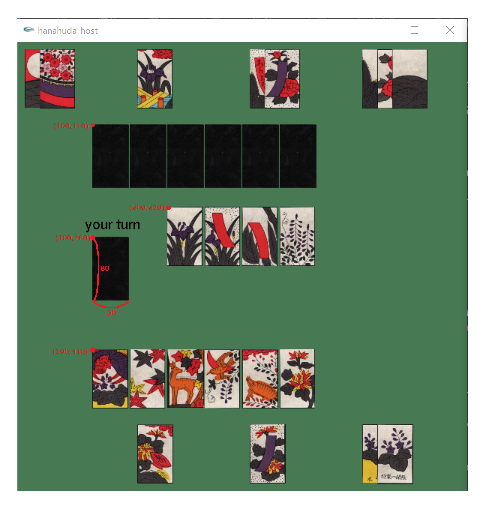
\includegraphics[scale=1.5]{./img/xy.eps}
    \caption{札の描画位置}
    \label{xy}
    \end{figure}

    キーボード入力はリスト\ref{keyboard}に示す関数で処理している. ゲームの進行状況を表すstatusが4のときのみキーボード入力を受け付けるようにしている.
    入力文字がyのときこいこいを表すためのフラグmykoikoiもしくはpeerkoikoiを1にして, 入力文字がnのとき, あがりを表すためフラグを0にしている.
    \begin{lstlisting}[basicstyle=\ttfamily\footnotesize, frame=single,label=keyboard,caption=キーボード入力の処理]
// キーボード入力の処理
void Keyboard(unsigned char key,int x,int y){
    if(status==4){
        if(key=='y'){ // こいこいするとき
            if(role==0){
                mykoikoi=1;
            }else{
                peerkoikoi=1;
            }
        }else if(key=='n'){ // こいこいしないとき
            if(role==0){
                mykoikoi=0;
            }else{
                peerkoikoi=0;
            }
        }

    }
}
    \end{lstlisting}

    \subsubsection{役の処理}
    役の処理は手札から出した札と山札からめくった札の処理が完了した後で実行される. リスト\ref{yaku}に示すように
    役の処理は役ができたかチェックするcheckYaku関数, でき役の得点を計算するcalcPoint関数, 役の表示を行うprintYaku関数
    の3つで構成されている. checkYaku関数は自分の所持している札の1枚ずつについて役に該当するかどうかチェックして役に該当すればフラグを
    立てる処理を行っている. 役のフラグはまとめて配列myyaku(親)と配列peeryaku(子)に格納される. calcPoint関数は配列myyakuまたは配列peeryakuの
    フラグをもとに得点を計算する関数である. 役に対する得点はhanahuda.cの配列pointlistに定義されている. printYaku関数はcalPoint関数の計算結果をもとに
    役をコンソールに表示する関数である. またこの関数で相手がこいこいしているときに得点2倍や7点以上2倍の計算を行ってコンソールに表示している.
    \begin{lstlisting}[basicstyle=\ttfamily\footnotesize, frame=single,label=yaku,caption=役の処理]
// 役のチェック
void checkYaku(void){
    int i,num;
    int checkkou=0;
    int flgrain=0; // 雨の光札用フラグ
    int hanami=0;
    int tukimi=0;
    int inosikacho=0;
    int akatan=0;
    int aotan=0;
    int tane=0;
    int tan=0;
    int kasu=0;
    if(role==0){
        for(i=0;i<mygetcard_num;i++){
        // 光札の数をカウント
        if(cards[mygetcard[i]].rank==4){
            // 雨かどうか
            if(cards[mygetcard[i]].month==11){
                flgrain=1;
            }
            checkkou++;
        }
        // 盃をチェック
        if((cards[mygetcard[i]].month==9)&&(cards[mygetcard[i]].rank==3)){
            hanami++;
            tukimi++;
            kasu++;
        }
        // 花見チェック
        if((cards[mygetcard[i]].month==3)&&(cards[mygetcard[i]].rank==4)){
            hanami++;
        }
        // 月見チェック
        if((cards[mygetcard[i]].month==8)&&(cards[mygetcard[i]].rank==4)){
            tukimi++;
        }
        // 猪鹿蝶チェック
        // 猪
        if((cards[mygetcard[i]].month==7)&&(cards[mygetcard[i]].rank==3)){
            inosikacho++;
        }
        // 鹿
        if((cards[mygetcard[i]].month==10)&&(cards[mygetcard[i]].rank==3)){
            inosikacho++;
        }
        // 蝶
        if((cards[mygetcard[i]].month==6)&&(cards[mygetcard[i]].rank==3)){
            inosikacho++;
        }

        // 赤短チェック
        if((cards[mygetcard[i]].month==1)&&(cards[mygetcard[i]].rank==2)){
            akatan++;
        }
        if((cards[mygetcard[i]].month==2)&&(cards[mygetcard[i]].rank==2)){
            akatan++;
        }
        if((cards[mygetcard[i]].month==3)&&(cards[mygetcard[i]].rank==2)){
            akatan++;
        }

        // 青短チェック
        if((cards[mygetcard[i]].month==6)&&(cards[mygetcard[i]].rank==2)){
            aotan++;
        }
        if((cards[mygetcard[i]].month==9)&&(cards[mygetcard[i]].rank==2)){
            aotan++;
        }
        if((cards[mygetcard[i]].month==10)&&(cards[mygetcard[i]].rank==2)){
            aotan++;
        }
        // 取得した札の枚数をカウント
        if(cards[mygetcard[i]].rank==3){
            tane++;
        }
        if(cards[mygetcard[i]].rank==2){
            tan++;
        }
        if(cards[mygetcard[i]].rank==1){
            kasu++;
        }
        }
       // 配列に役を格納
        if(checkkou==5){  // 五光 
            myyaku[0]=1; 
            myyaku[1]=0; // 四光, 雨四光, 三光を破棄
            myyaku[2]=0;
            myyaku[3]=0;
        }
        if((checkkou==4)&&(flgrain==0)){ // 四光
            myyaku[1]=1;
            myyaku[2]=0;
            myyaku[3]=0;  // 三光を破棄
        }
        if((checkkou==4)&&(flgrain==1)){ // 雨四光 
            myyaku[1]=0;
            myyaku[2]=1;
            myyaku[3]=0;  // 三光を破棄
        }
        if((checkkou==3)&&(flgrain==0)){ myyaku[3]=1; } // 三光
        if(hanami==2){ myyaku[4]=1;} // 花見で一杯
        if(tukimi==2){ myyaku[5]=1;} // 月見で一杯
        if(inosikacho==3){ myyaku[6]=1;} // 猪鹿蝶
        if(akatan==3){ myyaku[7]=1;} // 赤短
        if(aotan==3){ myyaku[8]=1;} // 青短
        if(tane>=5){// タネ 
            myyaku[9]=tane-4;
        }else{
            myyaku[9]=0;
        }
        if(tan>=5){ // タン 
            myyaku[10]=tan-4;
        }else{
            myyaku[10]=0;
        }
        if(kasu>=10){ // カス
            myyaku[11]=kasu-9;
        }else{
            myyaku[11]=0;
        }
    }else{
        for(i=0;i<peergetcard_num;i++){
        // 光札の数をカウント
        if(cards[peergetcard[i]].rank==4){
            // 雨かどうか
            if(cards[peergetcard[i]].month==11){
                flgrain=1;
            }else{
                checkkou++;
            }
        }
        // 盃をチェック
        if((cards[peergetcard[i]].month==9)&&(cards[peergetcard[i]].rank==3)){
            hanami++;
            tukimi++;
        }
        // 花見チェック
        if((cards[peergetcard[i]].month==3)&&(cards[peergetcard[i]].rank==4)){
            hanami++;
        }
        // 月見チェック
        if((cards[peergetcard[i]].month==8)&&(cards[peergetcard[i]].rank==4)){
            tukimi++;
        }
        // 猪鹿蝶チェック
        // 猪
        if((cards[peergetcard[i]].month==7)&&(cards[peergetcard[i]].rank==3)){
            inosikacho++;
        }
        // 鹿
        if((cards[peergetcard[i]].month==10)&&(cards[peergetcard[i]].rank==3)){
            inosikacho++;
        }
        // 蝶
        if((cards[peergetcard[i]].month==6)&&(cards[peergetcard[i]].rank==3)){
            inosikacho++;
        }

        // 赤短チェック
        if((cards[peergetcard[i]].month==1)&&(cards[peergetcard[i]].rank==2)){
            akatan++;
        }
        if((cards[peergetcard[i]].month==2)&&(cards[peergetcard[i]].rank==2)){
            akatan++;
        }
        if((cards[peergetcard[i]].month==3)&&(cards[peergetcard[i]].rank==2)){
            akatan++;
        }

        // 青短チェック
        if((cards[peergetcard[i]].month==6)&&(cards[peergetcard[i]].rank==2)){
            aotan++;
        }
        if((cards[peergetcard[i]].month==9)&&(cards[peergetcard[i]].rank==2)){
            aotan++;
        }
        if((cards[peergetcard[i]].month==10)&&(cards[peergetcard[i]].rank==2)){
            aotan++;
        }
        // 取得した札の枚数をカウント
        if(cards[peergetcard[i]].rank==3){
            tane++;
        }
        if(cards[peergetcard[i]].rank==2){
            tan++;
        }
        if(cards[peergetcard[i]].rank==1){
            kasu++;
        }
        }
        // 配列に役を格納
        if(checkkou==5){  // 五光 
            peeryaku[0]=1; 
            peeryaku[1]=0; // 四光, 雨四光, 三光を破棄
            peeryaku[2]=0;
            peeryaku[3]=0;
        }
        if((checkkou==4)&&(flgrain==0)){ // 四光
            peeryaku[1]=1;
            peeryaku[2]=0;
            peeryaku[3]=0;  // 三光を破棄
        }
        if((checkkou==4)&&(flgrain==1)){ // 雨四光 
            peeryaku[1]=0;
            peeryaku[2]=1;
            peeryaku[3]=0;  // 三光を破棄
        }
        if((checkkou==3)&&(flgrain==0)){ peeryaku[3]=1; } // 三光
        if(hanami==2){ peeryaku[4]=1;} // 花見で一杯
        if(tukimi==2){ peeryaku[5]=1;} // 月見で一杯
        if(inosikacho==3){ peeryaku[6]=1;} // 猪鹿蝶
        if(akatan==3){ peeryaku[7]=1;} // 赤短
        if(aotan==3){ peeryaku[8]=1;} // 青短
        if(tane>=5){// タネ 
            peeryaku[9]=tane-4;
        }else{
            peeryaku[9]=0;
        }
        if(tan>=5){ // タン 
            peeryaku[10]=tan-4;
        }else{
            peeryaku[10]=0;
        }
        if(kasu>=10){ // カス
            peeryaku[11]=kasu-9;
        }else{
            peeryaku[11]=0;
        }
    }
}

// 得点の計算
int calcPoint(void){
    int point=0;
    int i;
    for(i=0;i<YAKU_NUM;i++){
        if(role==0){
            point+=myyaku[i]*pointlist[i];
        }else{
            point+=peeryaku[i]*pointlist[i];
        }
    }
    return point;
}

// 役の表示
void printYaku(void){
    int i,point;
    printf("---------------\n");
    for(i=0;i<YAKU_NUM;i++){
        if(role==0){
            if(myyaku[i]!=0){
                printf("%s : %d点\n", yakuname[i],pointlist[i]*myyaku[i]);
            }
        }else{
            if(peeryaku[i]!=0){
                printf("%s : %d点\n", yakuname[i],pointlist[i]*peeryaku[i]);
            }
        }
    }
    point=calcPoint();

    if(role==0){
        if(peerkoikoi==1){
            point*=2;
            printf("相手こいこい得点2倍 ×2\n");
        }
    }else{
        if(mykoikoi==1){
            point*=2;
            printf("相手こいこい得点2倍 ×2\n");
        }
    }

    if(point>=7){
        point*=2;
        printf("7点以上得点2倍 ×2\n");
    }

    printf("合計 : %d点\n",point);
}
    \end{lstlisting}

    \subsubsection{ゲームの進行処理}
    ゲームの進行処理を行うDisplayと, ウィンドウに札の描画を行う関数, パケットの送受信について説明する. リスト\ref{paintcard}にウィンドウに札の描画を行う関数
    を示す. PutSprite関数は「Springs of C 楽しく身につくプログラミング」\cite{SC}定義されている画像を描画する関数を拡大縮小できるように改良したものである. PaintCards関数は
    図\ref{xy}の座標に従って札を描画し, マウスと重なっている手札または場札を赤で囲み, 選択されている札を青で囲む処理を行う.
    \begin{lstlisting}[basicstyle=\ttfamily\footnotesize, frame=single,label=paintcard,caption=札の描画を行う関数]
// (x,y)に大きさscaleの画像を表示
void PutSprite(int num, int x, int y, pngInfo *info,double scale)
{
    int w, h;  //  テクスチャの幅と高さ

    w = info->Width*scale;   //  テクスチャの幅と高さを取得する
    h = info->Height*scale;

    glPushMatrix();
    glEnable(GL_TEXTURE_2D);
    glBindTexture(GL_TEXTURE_2D, num);
    glColor4ub(255, 255, 255, 255);

    glBegin(GL_QUADS);  //  幅w, 高さhの四角形

    glTexCoord2i(0, 0); 
    glVertex2i(x, y);

    glTexCoord2i(0, 1);
    glVertex2i(x, y + h);

    glTexCoord2i(1, 1);
    glVertex2i(x + w, y + h);

    glTexCoord2i(1, 0);
    glVertex2i(x + w, y);

    glEnd();

    glDisable(GL_TEXTURE_2D);
    glPopMatrix();
}

// 札を描画
void PaintCards(void){
    int i,j,num;
    int x,y;
    // 場の札を描画
    x=200;
    y=220;

    // 場を描画
    for(i=0;i<place_num;i++){
        PutSprite(cardimg[place[i]],x,y,&cardinfo[place[i]],0.5);
        x+=50;
        if(i!=0 && i%6==5){
            y+=80;
            x=200;
        }
    }

    // 山札を描画
    PutSprite(cardimg[ALL_CARD-1],100,260,&cardinfo[ALL_CARD-1],0.5);

    // 自分の手札を描画
    x=100;
    y=410;
    if(role==0){
        num=mycard_num;
    }else{
        num=peercard_num;
    }
    for(i=0;i<num;i++){
            if(role==0){
                PutSprite(cardimg[mycard[i]],x,y,&cardinfo[mycard[i]],0.5);
            }else{
                PutSprite(cardimg[peercard[i]],x,y,&cardinfo[peercard[i]],0.5);
            }
        x+=50;
    }

    // 相手の手札を裏面にして描画
    x=100;
    y=110;
    if(role==0){
        num=peercard_num;
    }else{
        num=mycard_num;
    }
    for(i=0;i<num;i++){
        PutSprite(cardimg[ALL_CARD-1],x,y,&cardinfo[ALL_CARD-1],0.5);
        x+=50;
    }

    y=510;
    x=10;
    // 自分の持ち札を描画
    if(role==0){
        num=mygetcard_num;
    }else{
        num=peergetcard_num;
    }    
    for(i=4;i>=1;i--){ // 札の種類別に
        for(j=0;j<num;j++){
            if(role==0){
                if(cards[mygetcard[j]].rank==i){
                    PutSprite(cardimg[mygetcard[j]],x,y,&cardinfo[mygetcard[j]],0.5);
                    x+=20;
                }
            }else{
                if(cards[peergetcard[j]].rank==i){
                    PutSprite(cardimg[peergetcard[j]],x,y,&cardinfo[peergetcard[j]],0.5);
                    x+=20;
                }
            }
        }
        x=10+150*(5-i);
    }

    y=10;
    x=10;
    // 相手の持ち札を描画
    if(role==0){
        num=peergetcard_num;
    }else{
        num=mygetcard_num;
    }    
    for(i=4;i>=1;i--){ // 札の種類別に
        for(j=0;j<num;j++){
            if(role==1){
                if(cards[mygetcard[j]].rank==i){
                    PutSprite(cardimg[mygetcard[j]],x,y,&cardinfo[mygetcard[j]],0.5);
                    x+=20;
                }
            }else{
                if(cards[peergetcard[j]].rank==i){
                    PutSprite(cardimg[peergetcard[j]],x,y,&cardinfo[peergetcard[j]],0.5);
                    x+=20;
                }
            }
        }
        x=10+150*(5-i);
    }

    if(status==0){
        if(turn==0){
            if(role==0){
                if(selectedCard!=-1){
                    surroundCard(100+selectedCard*50,410,255,0,0);
                }
                if(clickedCard!=-1){
                    surroundCard(100+clickedCard*50,410,0,0,255);
                }
                if(selectedPlaceCard!=-1){
                    //下段
                    if(selectedPlaceCard>=6){
                        surroundCard(200+(selectedPlaceCard-6)*50,300,255,0,0);
                    }else{ // 上段
                        surroundCard(200+selectedPlaceCard*50,220,255,0,0);
                    }
                }
                if(clickedPlaceCard!=-1){
                    //下段
                    if(clickedPlaceCard>6){
                        surroundCard(200+(clickedPlaceCard-6)*50,300,0,0,255);
                    }else{ // 上段
                        surroundCard(200+clickedPlaceCard*50,220,0,0,255);
                    }            
                }
            }
        }else{
            if(role==1){
                if(selectedCard!=-1){
                    surroundCard(100+selectedCard*50,410,255,0,0);
                }
                if(clickedCard!=-1){
                    surroundCard(100+clickedCard*50,410,0,0,255);
                }
                if(selectedPlaceCard!=-1){
                    //下段
                    if(selectedPlaceCard>=6){
                        surroundCard(200+(selectedPlaceCard-6)*50,300,255,0,0);
                    }else{ // 上段
                        surroundCard(200+selectedPlaceCard*50,220,255,0,0);
                    }
                }
                if(clickedPlaceCard!=-1){
                    //下段
                    if(clickedPlaceCard>=6){
                        surroundCard(200+(clickedPlaceCard-6)*50,300,0,0,255);
                    }else{ // 上段
                        surroundCard(200+clickedPlaceCard*50,220,0,0,255);
                    }            
                }
            }
        }
    }
}
    \end{lstlisting}

    次に同期通信で送受信するパケットの内容について説明する. サーバー側とクライアント側で同じデッキを共有するために
    パケットを送受信する必要がある. 送受信するパケットはint型の長さ158の配列である. パケットの内容は図\ref{packet}に示す通りである.

    \begin{figure}[H]
    \centering
    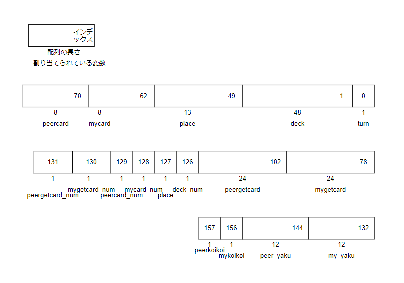
\includegraphics[scale=2.0]{./img/packet.eps}
    \caption{パケットの内容}
    \label{packet}
    \end{figure}

    図\ref{packet}に示したように送受信するパケットdataは複数の配列や変数から構成されるため, 値の入出力をまとめて行う関数を作成した.
    リスト\ref{packetattach}にパケットの送受信の処理を行う関数を示す. setPacket関数が引数で受け取ったdataに図\ref{packet}に示した
    パケットの内容をセットする関数, getPacket関数が受信したパケットの内容を配列や変数に代入する関数である.
    \begin{lstlisting}[basicstyle=\ttfamily\footnotesize, frame=single,label=packetattach,caption=パケットの処理]
// 送信するパケットの設定
void setPacket(int *data){
    int i,j;
    for(i=0;i<17;i++){
        if(i==0){ // turn
            data[packet_sep[i]]=turn;
        }else if(i==1){
            for(j=0;j<CARD_NUM;j++){
                data[packet_sep[i]+j] = deck[j];
            }               
        }else if(i==2){ // place
            for(j=0;j<PLACE_MAX;j++){
                data[packet_sep[i]+j] = place[j];
            }           
        }else if(i==3){ // mycard 
            for(j=0;j<INIT_PLACE;j++){
                data[packet_sep[i]+j] = mycard[j];
            }
        }else if(i==4){ // peercard
            for(j=0;j<INIT_PLACE;j++){
                data[packet_sep[i]+j] = peercard[j];
            }                
        }else if(i==5){ // mygetcard
            for(j=0;j<CARD_NUM/2;j++){
                data[packet_sep[i]+j] = mygetcard[j];
            }    
        }else if(i==6){
            for(j=0;j<CARD_NUM/2;j++){ // peergetcard
                data[packet_sep[i]+j] = peergetcard[j];
            }            
        }else if(i==7){
            data[packet_sep[i]] = deck_num;
        }else if(i==8){
            data[packet_sep[i]] = place_num;
        }else if(i==9){
            data[packet_sep[i]] = mycard_num;
        }else if(i==10){
            data[packet_sep[i]] = peercard_num;
        }else if(i==11){
            data[packet_sep[i]] = mygetcard_num;
        }else if(i==12){
            data[packet_sep[i]] = peergetcard_num;
        }else if(i==13){
            for(j=0;j<YAKU_NUM;j++){ // myyaku
                data[packet_sep[i]+j] = myyaku[j];
            }              
        }else if(i==14){
            for(j=0;j<YAKU_NUM;j++){ // peeryaku
                data[packet_sep[i]+j] = peeryaku[j];
            }                
        }else if(i==15){
            data[packet_sep[i]] = mykoikoi;
        }else if(i==16){
            data[packet_sep[i]] = peerkoikoi;
        }
    }
}

// 受信したパケットの解読
void getPacket(int *data){
    int i,j;
    for(i=0;i<17;i++){
        if(i==0){ // turn
            turn = data[packet_sep[i]];
        }else if(i==1){
            for(j=0;j<CARD_NUM;j++){
                deck[j]=data[packet_sep[i]+j];
            }               
        }else if(i==2){ // place
            for(j=0;j<PLACE_MAX;j++){
                place[j] = data[packet_sep[i]+j];
            }           
        }else if(i==3){ // mycard 
            for(j=0;j<INIT_PLACE;j++){
                mycard[j] = data[packet_sep[i]+j];
            }
        }else if(i==4){ // peercard
            for(j=0;j<INIT_PLACE;j++){
                peercard[j] = data[packet_sep[i]+j];
            }                
        }else if(i==5){ // mygetcard
            for(j=0;j<CARD_NUM/2;j++){
                mygetcard[j] = data[packet_sep[i]+j];
            }    
        }else if(i==6){
            for(j=0;j<CARD_NUM/2;j++){ // peergetcard
                peergetcard[j] = data[packet_sep[i]+j];
            }            
        }else if(i==7){
            deck_num = data[packet_sep[i]];
        }else if(i==8){
            place_num = data[packet_sep[i]];
        }else if(i==9){
            mycard_num = data[packet_sep[i]];
        }else if(i==10){
            peercard_num = data[packet_sep[i]];
        }else if(i==11){
            mygetcard_num = data[packet_sep[i]];
        }else if(i==12){
            peergetcard_num = data[packet_sep[i]];
        }else if(i==13){
            for(j=0;j<YAKU_NUM;j++){ // myyaku
                myyaku[j]=data[packet_sep[i]+j];
            }              
        }else if(i==14){
            for(j=0;j<YAKU_NUM;j++){ // peeryaku
                peeryaku[j]=data[packet_sep[i]+j];
            }                
        }else if(i==15){
            mykoikoi=data[packet_sep[i]];
        }else if(i==16){
            peerkoikoi=data[packet_sep[i]];
        }
    }    
}
    \end{lstlisting}

    ゲームの進行処理を行うDisplay関数について説明する. リスト\ref{display}にDisplay関数のプログラムを示す. Display関数はゲームの進行状況を分ける
    statusという変数によって処理を分けている. status=0のとき, パケットの送受信を行う処理とマウスの入力を受け付ける処理を行っている. また, パケットの受信結果において
    どちらかが上がった場合にstatus=6(後述)に処理がジャンプする. パケットの送信はwrite関数, 受信はread関数で行っている. どちらの関数も引数にソケット, データ, データ長をもつ.
    データ長は配列の長さとint型の4byteを掛けた数を与えている. \\
     status=0の状態で手札の札と場の札が選択されるとマウスを扱う関数の処理によってstatus=1になる. status=1の処理は札の獲得と山札のめくりである.
    獲得した札を配列に格納した後で, 山札から一枚popする. popした札でとれる場札が無ければその札を場においてstatus=3にする. とれる札が1枚のときは
    その札を場からpopし, 配列に格納する. とれる札が2枚以上あるときは, よりレア度の高い札をとる処理を行う.  status=0の状態で手札の札のみが選択され
    マウスを扱う関数によってstatus=2になっているとき, その札を場に出して山札をめくる処理を行う.\\
     山札をめくる処理が完了するとstatus=3の処理が行われる. status=3の処理は役を判定して画面に表示する処理である. 役を判定する前に, 一つ前の役を
    とっておき, 役を判定した後で前の役と判定することで新しい役ができたか判定している. もし役ができていれば, status=4, できていなければstatus=5の処理を行う.
    status=4のとき画面に図\ref{koikoi}のポップアップを表示してキーボード入力を待つ. キーボード入力に応じてこいこいかあがりかを判定して, status=5の処理に進む.

    \begin{figure}[H]
    \centering
    \includegraphics[scale=1.5]{./img/koikoi.png}
    \caption{ポップアップ表示}
    \label{koikoi}
    \end{figure}

    status=5のとき, ターン終了処理として, クリック選択を初期化し, turnを切り替える. そしてパケットを送信してこいこいのときstatus=0, そうでないときstatus=6の処理を行う.
    このタイミングで相手にパケットを送信することでターンが入れ替わるのと同時にデータの同期がまとめて行われる. status=6のとき役と勝敗を表示してゲームを終了する処理を行う.
    status=5でパケットを交換しているためターン交代時にどちらかのkoikoiフラグが0になっていればprintYaku関数で役を表示して勝敗を表示できる. 最後にstatus=7, つまり何も処理をしない
    状態にする. ゲーム終了時にexit関数を実行しないのは良い役が出来た時にスクリーンショットを取ることができるためである.

    \begin{lstlisting}[basicstyle=\ttfamily\footnotesize, frame=single,label=display,caption=Display関数]
// メインループ
void Display(void){
    int data[DATA_LENGTH];
    char dispstr[100];
    int r,i,j;
    int tmp;
    int tmpcard;
    int tmpyaku[YAKU_NUM];

    // 描画クリア
    glClear(GL_COLOR_BUFFER_BIT);
    // 札描画
    PaintCards();
    // 札選択
    if(status==0){ // 同期処理と札選択
        if(turn==0){
            if(role==0){
                setPacket(data);
                write(hanahuda_soc,&data[0],4*DATA_LENGTH);
                glColor3ub(0,0,0);
                glRasterPos2i(90,250);
                sprintf(dispstr,"your turn");
                for(i=0;i<strlen(dispstr);i++){
                    glutBitmapCharacter(GLUT_BITMAP_HELVETICA_18,dispstr[i]);
                }
            }else{
                read(hanahuda_soc,&data[0],4*DATA_LENGTH);
                getPacket(data);
                glColor3ub(0,0,0);
                glRasterPos2i(110,250);
                sprintf(dispstr,"wait");
                for(i=0;i<strlen(dispstr);i++){
                    glutBitmapCharacter(GLUT_BITMAP_HELVETICA_18,dispstr[i]);
                }
            }
         }else{
            if(turn==1){
                if(role==1){
                    setPacket(data);
                    write(hanahuda_soc,&data[0],4*DATA_LENGTH);
                    glColor3ub(0,0,0);
                    glRasterPos2i(90,250);
                    sprintf(dispstr,"your turn");
                    for(i=0;i<strlen(dispstr);i++){
                        glutBitmapCharacter(GLUT_BITMAP_HELVETICA_18,dispstr[i]);
                    }
                }
                if(role==0){
                    read(hanahuda_soc,&data[0],4*DATA_LENGTH);
                    getPacket(data);
                    glColor3ub(0,0,0);
                    glRasterPos2i(110,250);
                    sprintf(dispstr,"wait");
                    for(i=0;i<strlen(dispstr);i++){
                        glutBitmapCharacter(GLUT_BITMAP_HELVETICA_18,dispstr[i]);
                    }
                }    
            }
        }
        if((mykoikoi==0)||(peerkoikoi==0)){
            status=6;
        }
        if((mycard_num==0)&&(peercard_num==0)){
            status=6;
        }
    }else if(status==1){ // 手札から出した札で札が取れるとき
        // 場札の獲得
        r = popHandCard(clickedCard);
        pushgetCard(r);
        r = popPlace(clickedPlaceCard);
        pushgetCard(r);

        // 山札から出した札の処理
        r = popDeck();
        if(isGetPlace(r)==0){ // 取れる札がないとき
            pushPlace(r);
        }else if(isGetPlace(r)==1){ // 取れる札が1枚のとき
            pushgetCard(r);
            for(i=0;i<place_num;i++){
                if(cards[r].month==cards[place[i]].month){
                    r=popPlace(i);
                    break;
                }
            }
            pushgetCard(r);
        }else if(isGetPlace(r)>=2){ // 取れる札が2枚のとき
            tmp=0;
            for(i=0;i<place_num;i++){ // 得点の高い札を探索
                if(cards[place[i]].month==cards[r].month){ // rと月が一緒なら
                    if(tmp<cards[place[i]].rank){
                        tmpcard=i;
                        tmp=cards[place[i]].rank;
                    }
                }
            }
            pushgetCard(r);
            r = popPlace(tmpcard);
            pushgetCard(r);
        }
        status=3; // 役の処理へ
    }else if(status==2){ // 手札から出した札で札が取れないとき
        // 手札から1枚だす
        r = popHandCard(clickedCard);
        pushPlace(r); 

        // 山札から出した札の処理
        r = popDeck();
        if(isGetPlace(r)==0){ // 取れる札がないとき
            pushPlace(r);
        }else if(isGetPlace(r)==1){ // 取れる札が1枚のとき
            pushgetCard(r);
            for(i=0;i<place_num;i++){
                if(cards[r].month==cards[place[i]].month){
                    r=popPlace(i);
                    break;
                }
            }
            pushgetCard(r);
        }else if(isGetPlace(r)>=2){ // 取れる札が2枚のとき
            tmp=0;
            for(i=0;i<place_num;i++){ // 得点の高い札を探索
                if(cards[place[i]].month==cards[r].month){ // rと月が一緒なら
                    if(tmp<cards[place[i]].rank){
                        tmpcard=i;
                        tmp=cards[place[i]].rank;
                    }
                }
            }
            pushgetCard(r);
            r = popPlace(tmpcard);
            pushgetCard(r);
        }
        status=3; // 役の処理へ      
    }else if(status==3){ // 役の処理
    // 1つ前の役の和を計算
    tmp=0;
    if(role==0){
        for(i=0;i<YAKU_NUM;i++){
            tmpyaku[i]=myyaku[i];
        }
    }else{
        for(i=0;i<YAKU_NUM;i++){
            tmpyaku[i]=peeryaku[i];
        }
    }
    checkYaku();
    if(role==0){
        for(i=0;i<YAKU_NUM;i++){
            if(tmpyaku[i]!=myyaku[i]){
                tmp=1;
                break;
            }
        }
    }else{
        for(i=0;i<YAKU_NUM;i++){
            if(tmpyaku[i]!=peeryaku[i]){
                tmp=1;
                break;
            }
        }
    }    

    if(role==0){
        if(tmp==1){
            printYaku();
            mykoikoi=-1;
            status=4;
        }else{status=5;}   
    }else{
        if(tmp==1){
            printYaku();
            peerkoikoi=-1;
            status=4;
        }else{status=5;}
    }
    }else if(status==4){ // こいこいの処理
        if((turn==0)&&(role==0)){
            PutSprite(koikoiimg,200,200,&koikoiinfo,1);
        }else if((turn==1)&&(role==1)){
            PutSprite(koikoiimg,200,200,&koikoiinfo,1);
        }

        if(role==0){
            if(mykoikoi!=-1){
                status=5;
            }
        }else{
            if(peerkoikoi!=-1){ 
                status=5;
            }
        }
    }else if(status==5){ // ターン終了処理
        selectedCard=-1;
        clickedCard=-1;
        selectedPlaceCard=-1;
        clickedPlaceCard=-1;
        turn=1-turn;
        // パケット送信準備
        setPacket(data);
        write(hanahuda_soc,data,4*DATA_LENGTH);
        if(role==0){
            if(mykoikoi==0){
                status=6;
            }else{
                status=0;
            }
        }else{
            if(peerkoikoi==0){
                status=6;
            }else{
                status=0;
            }
        }
    }else if(status==6){ // ゲーム終了処理
        printYaku();
        if((mykoikoi!=0)&&(peerkoikoi!=0)){
            printf("引き分け\n");
        }
        if(mykoikoi==0){
            printf("親の勝ちです\n");
        }
        if(peerkoikoi==0){
            printf("子の勝ちです\n");
        }
        printf("ゲームを終了してください\n");
        status=7;
    }
    // 描画の反映
    glFlush(); 
}
    \end{lstlisting}

    \subsection{hanahuda.h}
    リスト\ref{hanahudah}にhanahuda.hのコードを示す.
    \begin{lstlisting}[basicstyle=\ttfamily\footnotesize, frame=single,label=hanahudah,caption=hanahuda.h]
#include <sys/types.h>
#include<GL/glut.h>
#include <GL/glpng.h>
#include "mylib.h"

#define PORT (in_port_t)50000 // ポート番号
#define HOSTNAME_LENGTH 64 // ホストネーム長
#define DATA_LENGTH 158 // 同期通信でやりとりするパケット長

#define WINDOW_W 600 // ウィンドウの横の長さ
#define WINDOW_H 600 // ウィンドウの縦の長さ
#define CARD_WIDTH 128 // 札の縦の長さ(読み込み時)
#define CARD_HEIGHT 256 // 札の横の長さ(読み込み時)
#define CARD_NUM 48 // 12*4
#define ALL_CARD 49 // 全札+裏面の札
#define MONTH 12 // 月の数
#define MONTH_CARD 4 // 1つの月の札の数
#define PLACE_MAX 13 // 場における最大札数
#define INIT_PLACE 8 // 最初の場の数
#define SHUFFLE_TIME 1000 // 山札をシャッフルする回数
#define YAKU_NUM 12 // 役の数

static int pointlist[YAKU_NUM] = {10,8,7,5,5,5,5,5,5,1,1,1}; // 役を取った時の得点
static int packet_sep[17] ={0,1,49,62,70,78,102,126,127,128,129,130,131,132,144,156,157}; 
// パケットの区切り目  
static GLuint cardimg[ALL_CARD]; // 札描画のための構造体
static pngInfo cardinfo[ALL_CARD]; // 札描画のための構造体
static GLuint koikoiimg; // こいこいポップアップの画像
static pngInfo koikoiinfo; // こいこいポップアップの画像

static char month[MONTH][4]={"jan","feb","mar","apr","may","jun",
                            "jul","aug","sep","oct","nov","dec"}; // 月の英語表記(略記)
static char yakuname[YAKU_NUM][20] = {"五光","四光","雨四光","三光","花見で一杯","月見で一杯",
                                    "猪鹿蝶","赤短","青短","タネ","タン","カス"}; // 役名

// 札の点数
static int cardrank[MONTH][4] ={{4,2,1,1}, // 松に鶴
                                {3,2,1,1}, // 梅にうぐいす
                                {4,2,1,1}, // 桜に幕
                                {3,2,1,1}, // 藤にほととぎす
                                {3,2,1,1}, // 菖蒲に八ツ橋
                                {3,2,1,1}, // 牡丹に蝶
                                {3,2,1,1}, // 萩に猪
                                {4,3,1,1}, // ススキに月・雁
                                {3,2,1,1}, // 菊に盃
                                {3,2,1,1}, // 紅葉に鹿
                                {4,3,2,1}, // 小野道風にカエル・柳にツバメ
                                {4,1,1,1}}; // 桐に鳳凰

// 札用の構造体
struct cardstruct{
    int month; // 1-12
    int num; // imgの番号
    int rank; //1-4, 4:光札,3:タネ札,2:短冊札,1:カス札
};
typedef struct cardstruct card;
// 札用の構造体の配列を定義
static card cards[CARD_NUM];

static int deck_num=0; // 次に出る山札配列のindex
static int deck[CARD_NUM]; // 山札
static int place_num=0; // 場に出ている札の数
static int place[PLACE_MAX]; // 場の配列
static int mycard_num=INIT_PLACE; //親の札の数
static int mycard[INIT_PLACE]; //親の札
static int peercard_num=INIT_PLACE; //子の札の数
static int peercard[INIT_PLACE]; //子の札 
static int role; // 親(0)か子(1)か
static int turn=0; // 誰のターンか
static int selectedCard=-1; // 選択中の手札の札の番号を保持
static int clickedCard=-1; // クリックした手札の札を保持 
static int selectedPlaceCard=-1; // 選択中の場札の札の番号を保持
static int clickedPlaceCard=-1; // クリックした場札の札の番号を保持
static int mygetcard_num=0; // 取得した札の枚数
static int mygetcard[CARD_NUM/2]; // 取得した札の番号の配列
static int peergetcard_num=0; // 子が取得した札の枚数
static int peergetcard[CARD_NUM/2]; // 子が取得した札の番号の配列
static int myyaku[YAKU_NUM]; // 取得した札
static int peeryaku[YAKU_NUM]; // 子が取得した札
static int mykoikoi=-1; // こいこいの状態
static int peerkoikoi=-1; // 子のこいこいの状態
static int hanahuda_soc; // ソケット
static int status=0; // ターンの進行状態

void Reshape(int,int);
void Timer(int);
void PutSprite(int,int,int,pngInfo *,double);
void readImg(void);
void array_init(void);
void card_init(void);
void shuffle(void);
void game_init(int,int);
int popDeck(void);
void pushPlace(int c);
int popPlace(int);
int popHandCard(int);
void pushgetCard(int);
int arrangeCard(void);
void surroundCard(int,int,int,int,int);
void PaintCards(void);
int calWhichPlacecard(int,int);
int calWhichMycard(int,int);
int isGetCard(int);
int isGetPlace(int);
void Keyboard(unsigned char,int,int);
void Mouse(int,int,int,int);
void PassiveMotion(int,int);
void checkYaku(void);
void printYaku(void);
int calcPoint(void);
void setPacket(int *data);
void getPacket(int *data);
void Display(void);
    \end{lstlisting}

    \subsection{Makefile}
    リスト\ref{makefile}にmainディレクトリのMakefileのコードを示す.
    \begin{lstlisting}[basicstyle=\ttfamily\footnotesize, frame=single,label=makefile,caption=Makefile]
MYLIBDIR = ../mylib
MYLIB    = $(MYLIBDIR)/mylib.a
CFLAGS   = -I$(MYLIBDIR)

CC = gcc
CCFLAGS = -Wall -I/usr/include/opengl
LD = gcc
LDFLAGS =
LIBS = -lglpng -lglut32 -lglu32 -lopengl32 -lm #myicon.o

all:	s c

s:		server.o hanahuda.o
		$(CC) -o $@ $^ $(MYLIB)	$(LIBS)	

c:		client.o hanahuda.o
		$(CC) -o $@ $^ $(MYLIB) $(LIBS)

server.o client.o:	hanahuda.h

clean:
		 $(RM) s c *.o *~
    \end{lstlisting}

    \section{実行結果}
    本章では実行結果としてマウスの処理, こいこい時の表示, ゲーム終了時の表示の3つについて述べる.
    \subsection{マウスの処理}
    マウス処理ができていることを確認する. マウス入力は, マウスが乗っている手札を赤, クリックした手札を青で囲む処理ができていることを確認する.
    まず, マウスが乗っている手札をが赤い四角形で囲まれることを確認する. 図\ref{selectred}に手札の上にマウスを乗せたときの画面表示を示す. スクリーンショットの関係で
    マウスが表示されていないが, マウスが乗っている右から3番目の手札が赤い四角形で囲まれていることがわかる.

    \begin{figure}[H]
    \centering
    \includegraphics[scale=1.0]{./img/select.eps}
    \caption{マウスが乗っている札が赤で囲まれることの確認}
    \label{selectred}
    \end{figure}

    次にクリックした札が青い四角形で囲まれることを確認する. 図\ref{clickblue}に札をクリックしたときの画面表示を示す. 場札に同じ月の札がある
    9月のタン札をクリックすると青い四角形で囲まれることが確認できた.

    \begin{figure}[H]
    \centering
    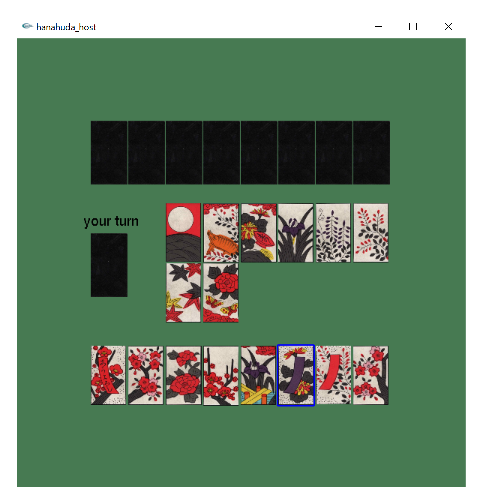
\includegraphics[scale=1.0]{./img/click.eps}
    \caption{札をクリックしたときの表示}
    \label{clickblue}
    \end{figure}

    \subsection{こいこい時の表示}
    こいこい時にウィンドウにはこいこいのポップアップ, コンソールには役が表示されることを確認する. 図\ref{koikoipopup}にこいこい時の
    画面とコンソールの表示を示す. 図\ref{koikoipopup}は親が月見で一杯の役を完成させたときのこいこいの表示である. 役が完成するとウィンドウに
    「こいこいしますか?」と表示され, コンソールに役と得点が表示されることが確認できる.
    \begin{figure}[H]
    \centering
    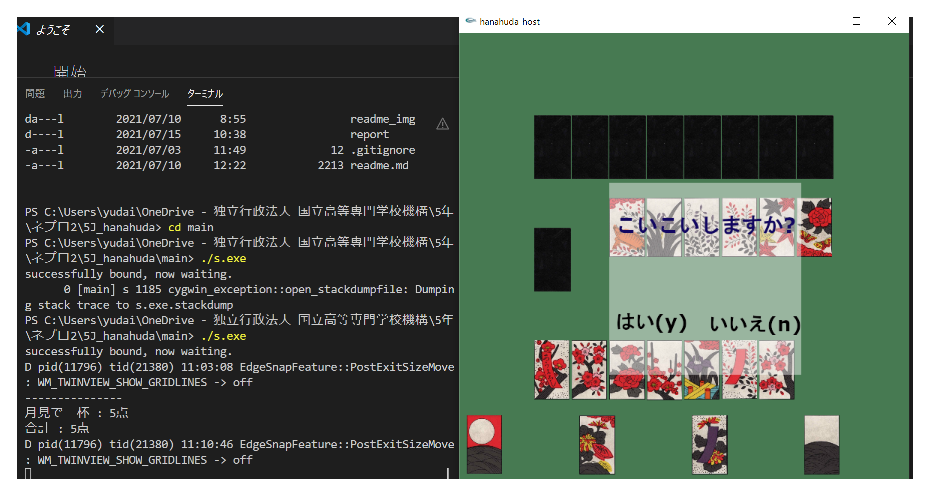
\includegraphics[scale=1.0]{./img/koikoi_popup.eps}
    \caption{こいこい時の表示}
    \label{koikoipopup}
    \end{figure}

    \subsection{ゲーム終了時の表示}
    ゲーム終了時のウィンドウとコンソール表示を確認する. ゲームが終了するとウィンドウにはそれまでの盤面が表示され, コンソールには自分側の得点と勝敗が表示される.
    図\ref{gameend}にゲーム終了時のウィンドウ表示を示す. 図\ref{clickblue}に示したようにプレイ中はターン中のプレイヤーの画面に「your turn」, もしくは「wait」
    と表示されるがゲーム終了時は何も表示されない. またコンソールには図\ref{gameendconsole}自分のでき役と得点が表示される. 図\ref{gameend}と
    図\ref{gameendconsole}の例では花見で一杯, 月見で一杯の役ができており, 加えて7点以上2倍によって合計20点の得点が表示されていることが読み取れる.

    \begin{figure}[H]
    \centering
    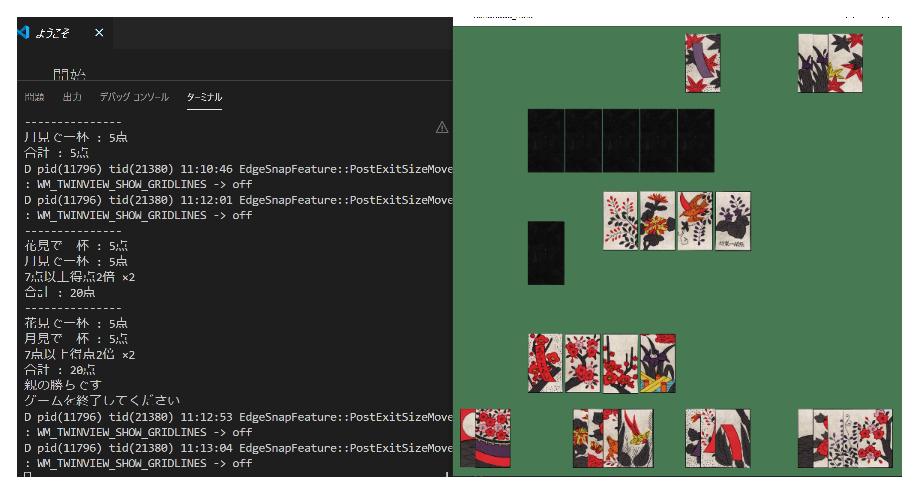
\includegraphics[scale=1.0]{./img/agari.eps}
    \caption{ゲーム終了時のウィンドウ}
    \label{gameend}
    \end{figure}

    \begin{figure}[H]
    \centering
    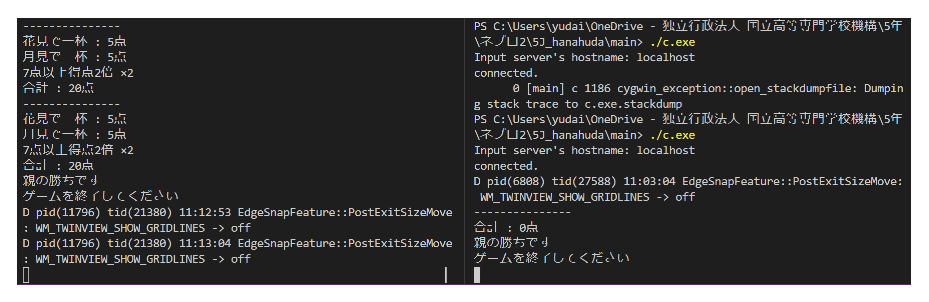
\includegraphics[scale=1.0]{./img/game_end.eps}
    \caption{ゲーム終了時のコンソール}
    \label{gameendconsole}
    \end{figure}

    \section{改善点・感想}
    ホストとクライアントが接続した後にstackdumpすることがあるが開発時間の関係でこのバグを取り切れなかったため改善したい. またlocalhostでは上手く動作したが, 
    別々の端末でs.exeとc.exeを実行すると強制終了する場合があるためこの問題も改善したい. 4年次のプログラミング演習でOpenGLを使用した桃太郎電鉄風のゲームを作成したが, 
    複数端末でプレイ出来ないかと考えていたが本課題を通してOpenGLとソケット通信を組み合わせられることが分かったため非常に面白かった. 

        \begin{thebibliography}{9}
          \bibitem{nintendo}  Nintendo,花札の歴史・遊び方,\url{hhttps://www.nintendo.co.jp/others/hanafuda_kabufuda/howtoplay/index.html} ,閲覧日2021年7月13日
          \bibitem{SC}  伊藤祥一, "Spring of C 楽しく身ににつくプログラミング",森北出版株式会社,2017年
        \end{thebibliography}
\end{document}